\documentclass[20 pts]{article}
\usepackage{xeCJK}
\usepackage{amsfonts}
\usepackage{amssymb}
\usepackage{amsmath}
\usepackage{bm}
\setCJKmainfont{SimSun}

\begin{document}
\begin{figure}
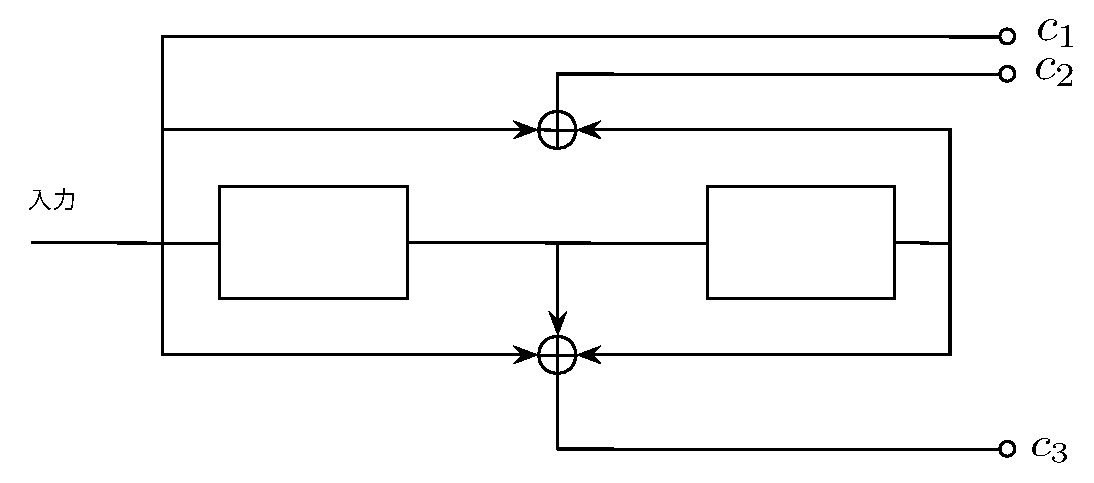
\includegraphics[width=15cm]{figure1.pdf}
\caption{K=3,k=1,n=2 畳み込み符号}
\label{図1}
\end{figure}%

\newpage
\begin{figure}
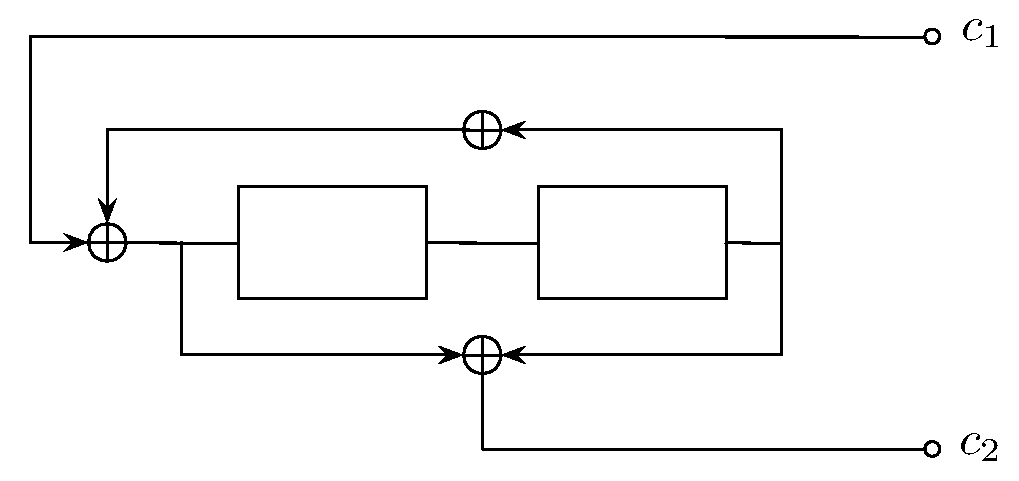
\includegraphics[width=15cm]{figure2.pdf}
\caption{再帰的系統的畳み込み(RSC)符号器,K=3,k=1,n=2}
\label{図2}
\end{figure}%

\begin{figure}
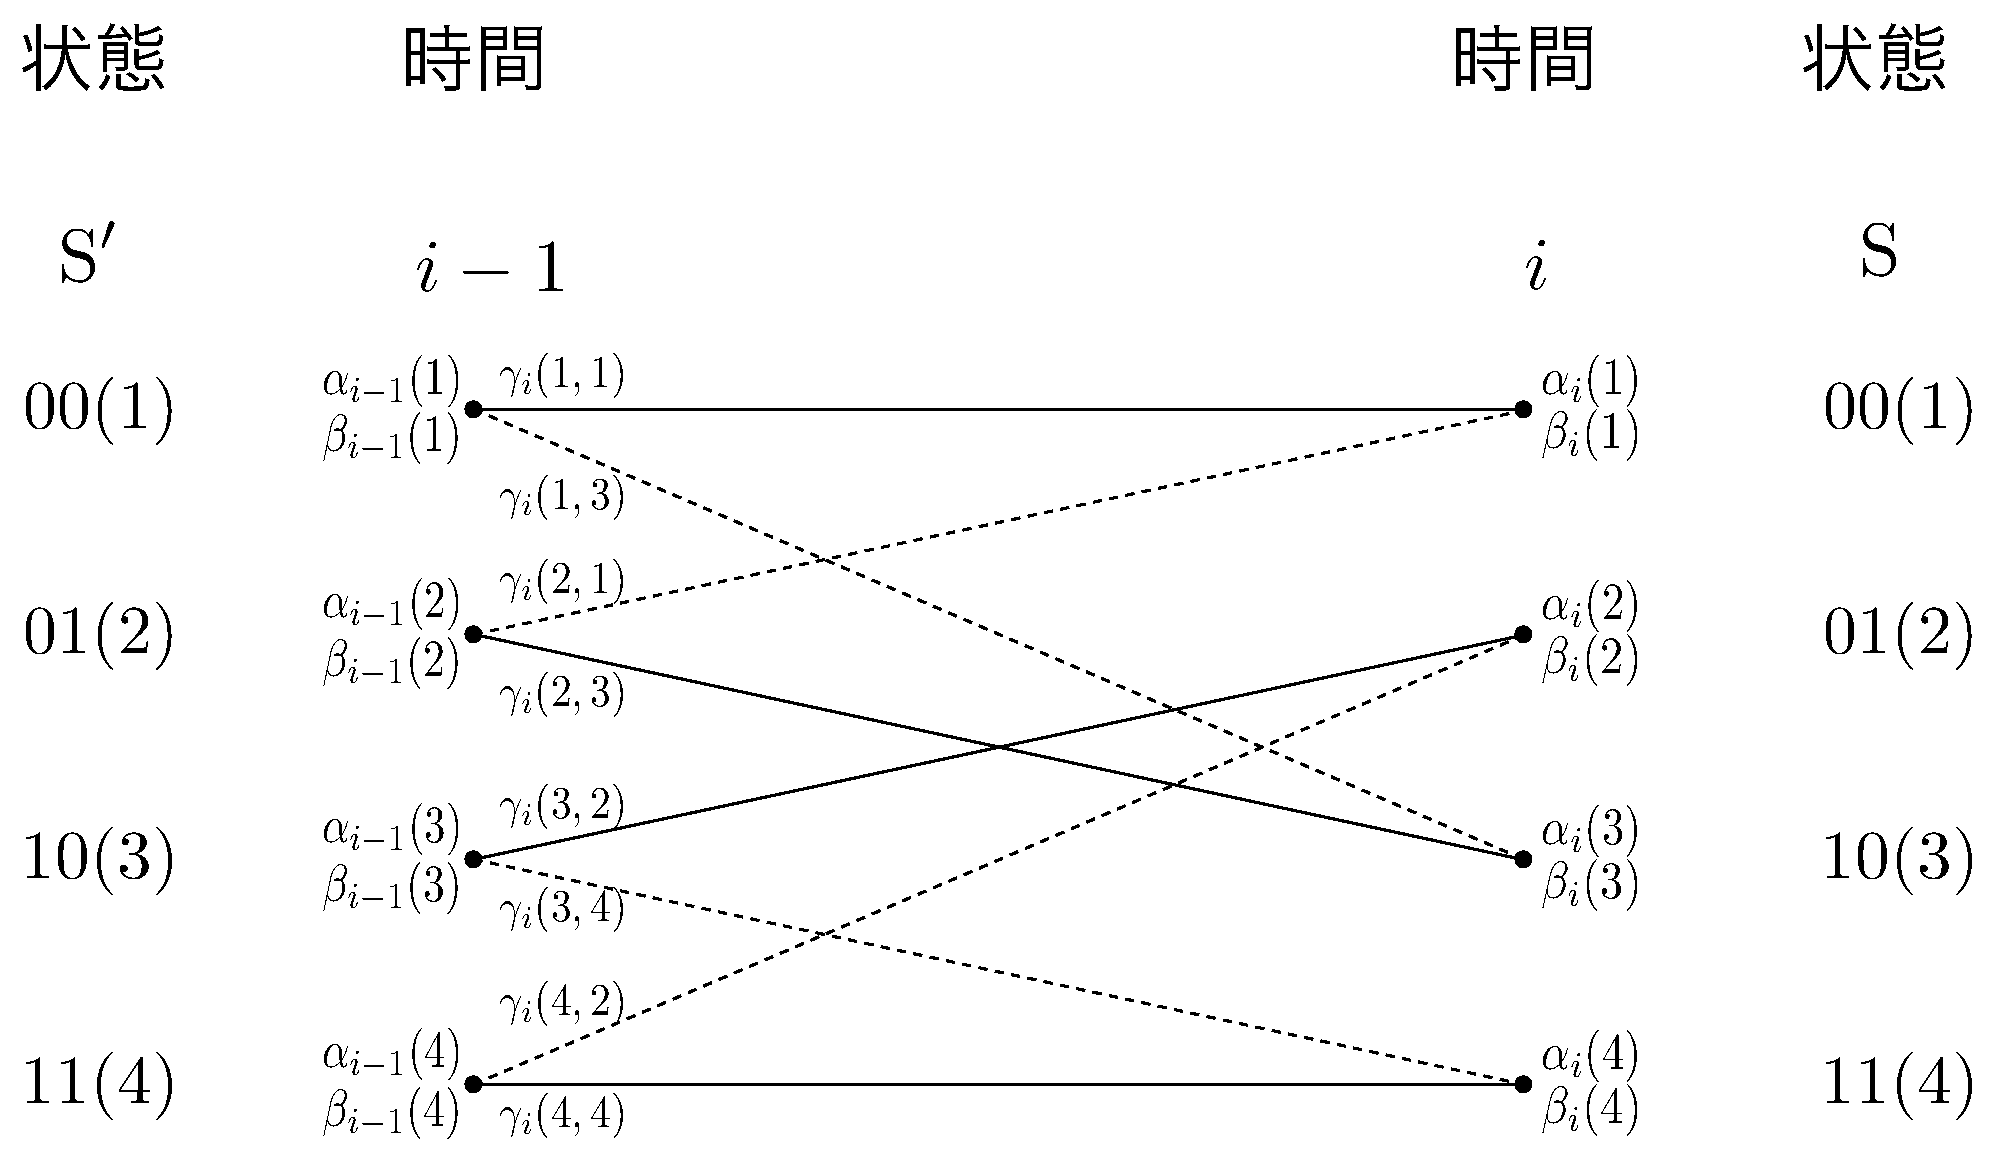
\includegraphics[width=15cm]{figure3.pdf}
\caption{$\alpha,\beta,\gamma$のtrellisラベル。再帰的系統的畳み込み(RSC)符号器,K=2,k=1,n=2,$g_1=1+D,g_2=1$}
\label{図2}
\end{figure}%


\newpage
\begin{figure}
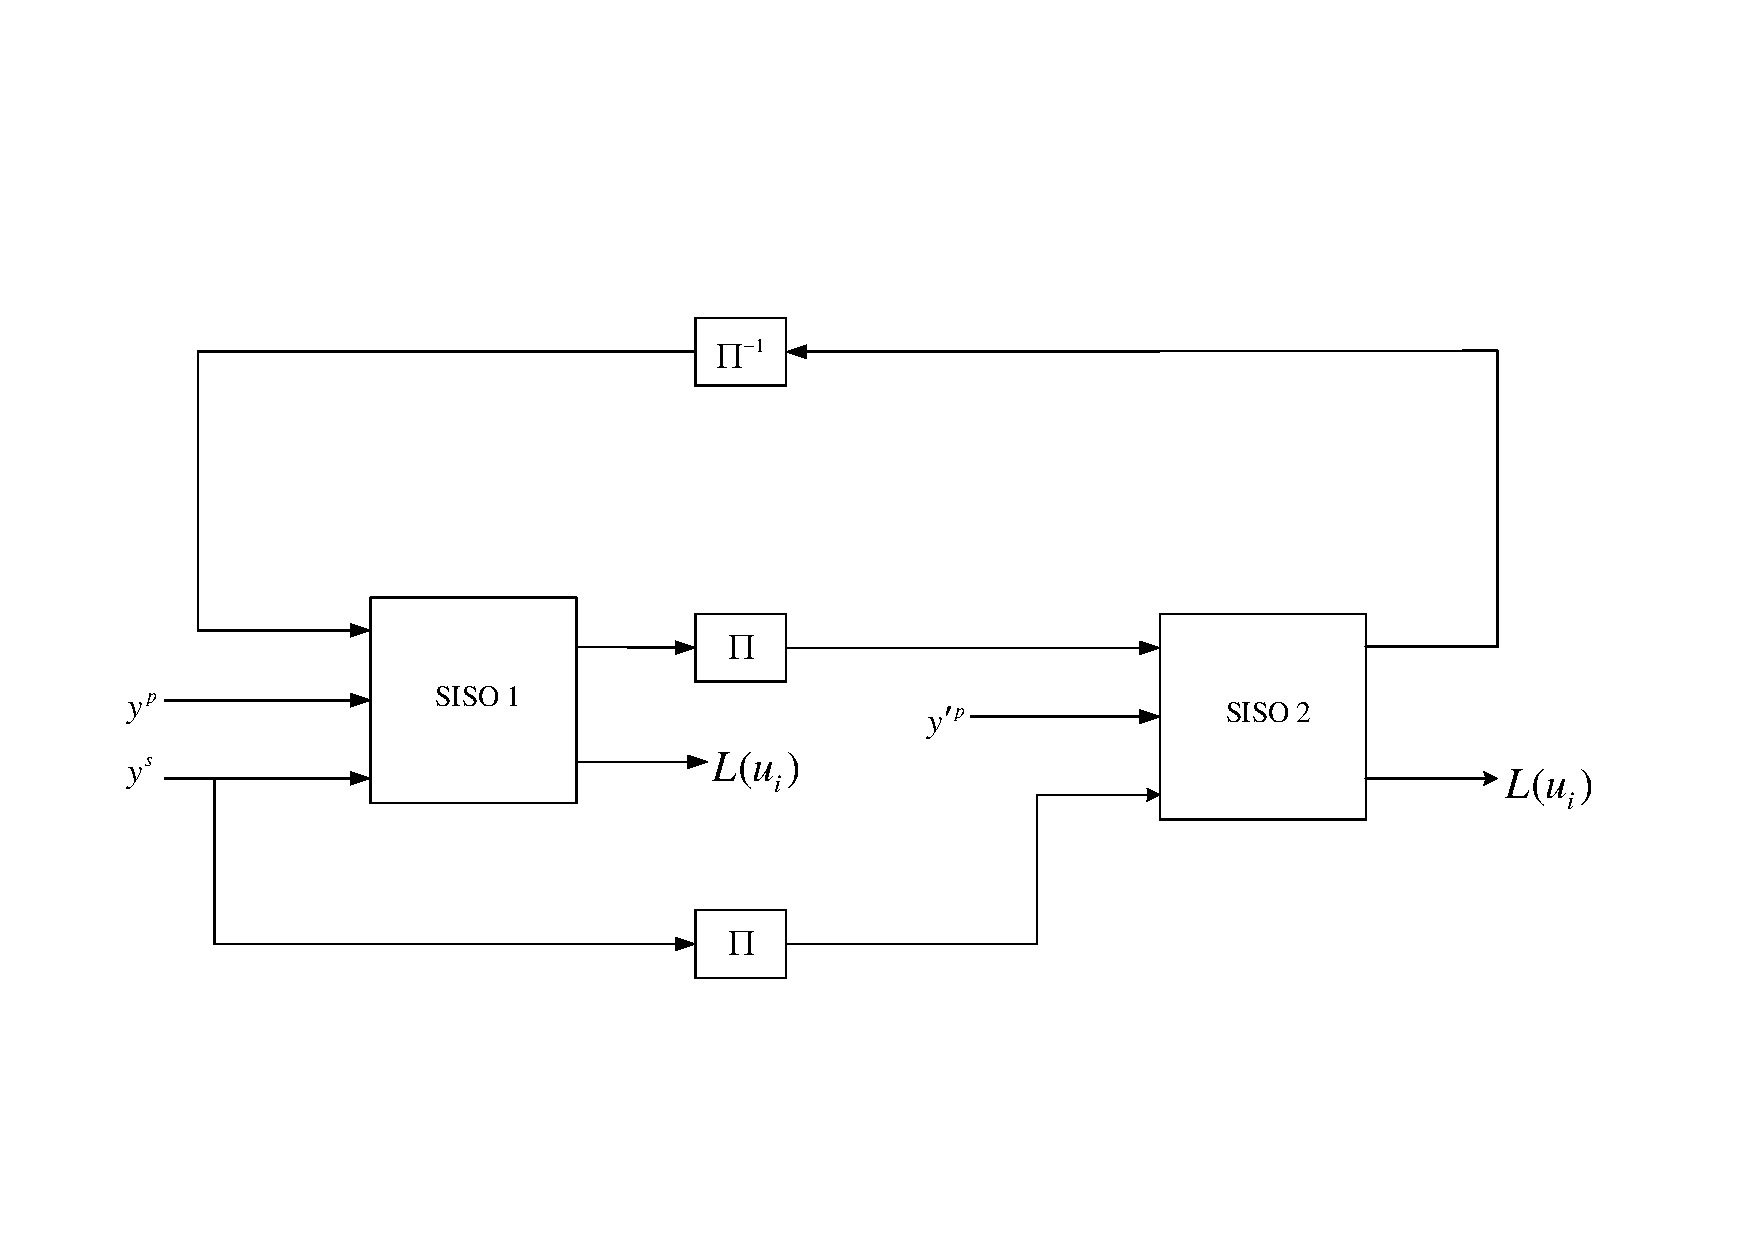
\includegraphics[width=15cm]{D1.pdf}
\caption{ターボ復号器}
\label{図2}
\end{figure}%

\begin{figure}
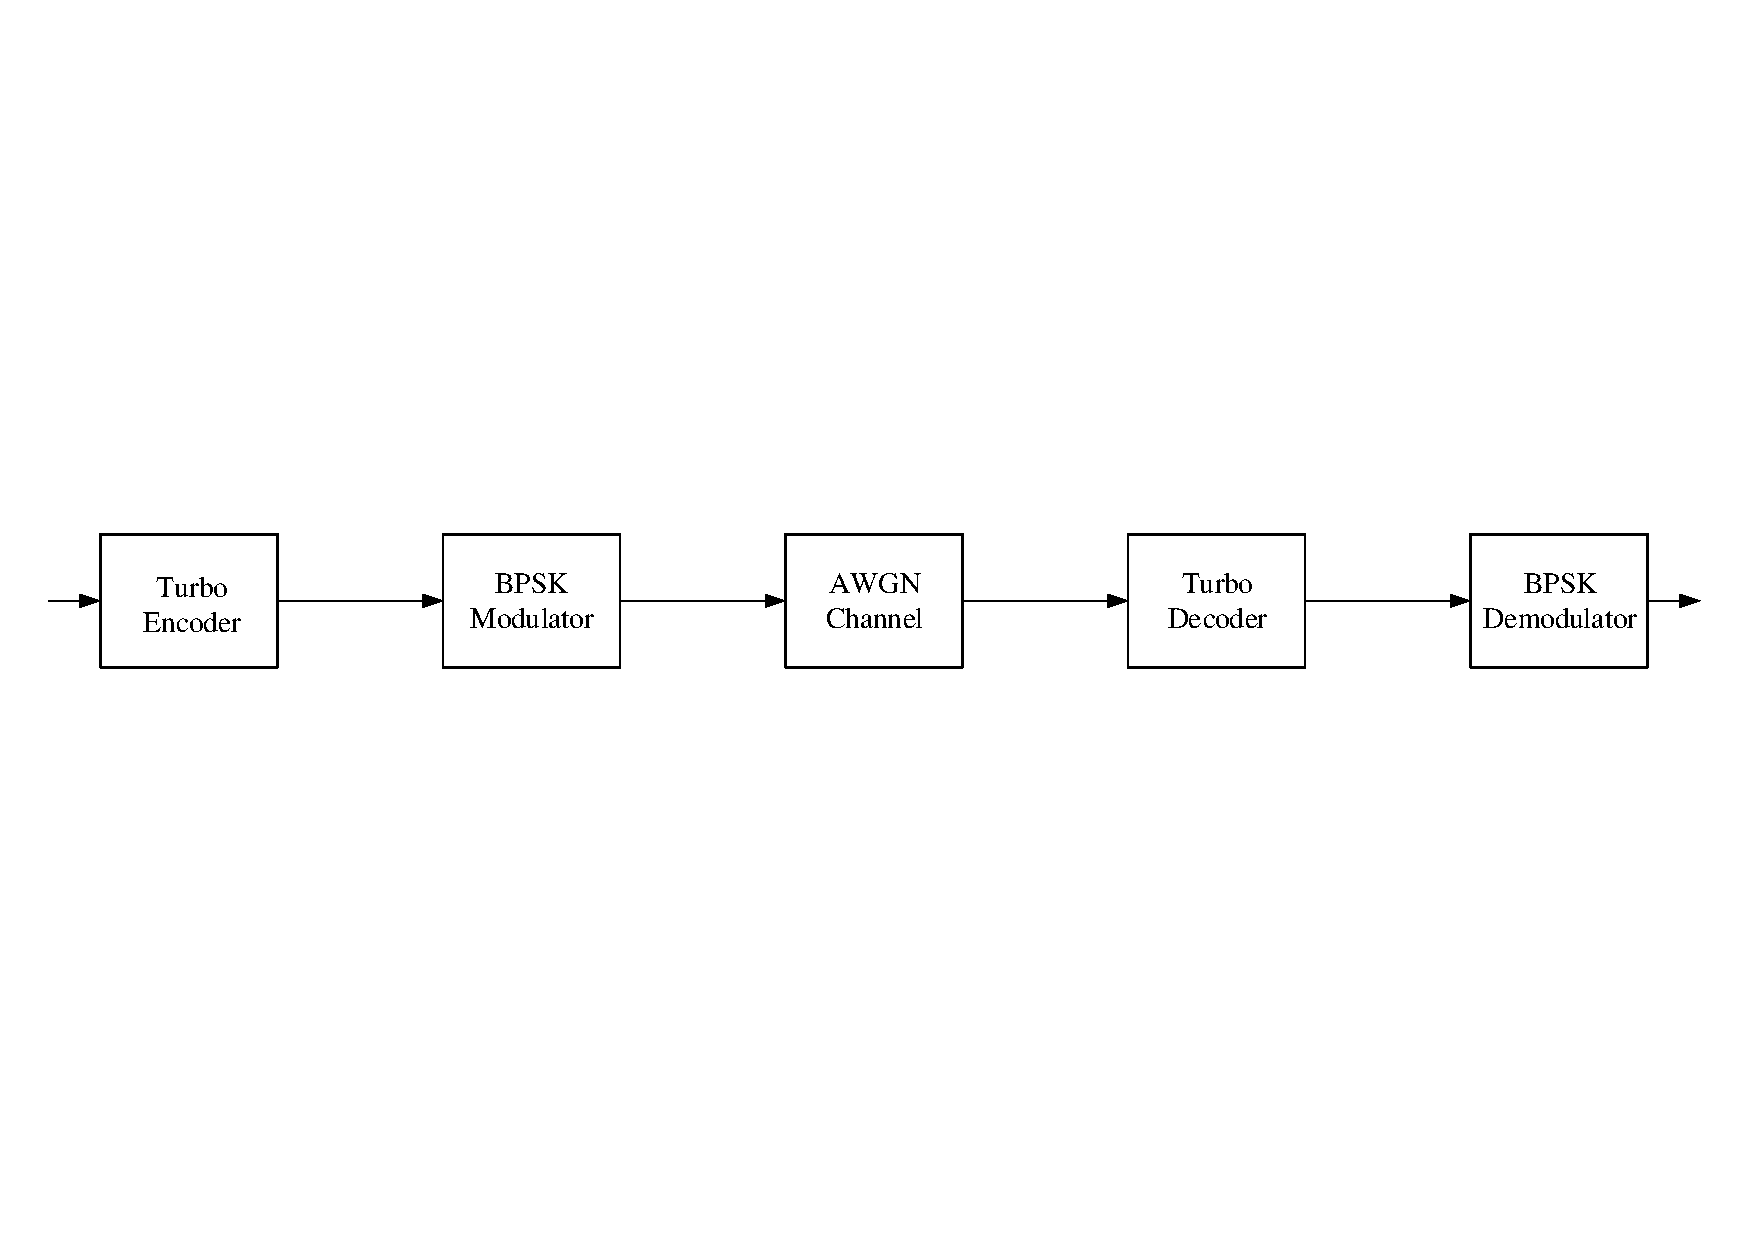
\includegraphics[width=15cm]{D2.pdf}
\caption{システムモデル}
\label{図2}
\end{figure}%

\end{document}